\part{Capítulo uno}
\graphicspath{ {1_Capitulo/img/portada/},{1_Capitulo/img/explicacion/},{1_Capitulo/img/ejemplos/} }

%----------------------------------------------------------------------------------------
%	CHAPTER 1
%----------------------------------------------------------------------------------------

\chapterimage{portada.jpg} % Chapter heading image

\chapter{Interés simple}
\section{Mapa Mental }
\begin{figure}[h]
	\centering
	\includegraphics[scale=0.5]{"Mapa Mental 1 V1.0.pdf"}
	\caption{Mapa mental interes simple}
\end{figure}
\newpage
\section{Fórmulas de capítulo}

\begin{spacing}{1.5}
	\begin{center}
		\begin{tabular}{ |p{6cm}|p{5cm}| p{4cm}|}
			\hline
			\rowcolor{orange!50}
			\begin{center}\textbf{Fórmula} \end{center} & \begin{center} \textbf{Nombre}\end{center}          & \begin{center} \textbf{Excel} \end{center} \\ \hline
			
			I = Pin                   & Valor interés simple               & TASA.INT(ni;nf;P)         \\ \hline
			
			F = P+I                   & Valor futuro                       & -                         \\ \hline
			
			P= $\frac{F}{1+ni }$      & Valor presente                     & -                         \\ \hline
			
			
			F= P(1+in)                & Valor futuro                       & -                         \\ \hline
			
			P= F(1-dn)                & Valor presente de un flujo futuro  & -                         \\ \hline
			
			F= P/(1-dn)               & Valor futuro de un flujo presente  & -                         \\ \hline
			
			VL= F(1-dn)               & Valor líquido dado un flujo futuro & -                         \\ \hline
		\end{tabular}
	\end{center}
\end{spacing}

\section{Introducción}
En este capítulo daremos definiciones y conceptos básicos utilizados en las finanzas, los cuales serán indispensables para el desarrollo de la guía. Este enfoque analítico nos permite la optimización de los recursos económicos, lo cual viene a ser el objetivo final de esta guía.

\section{Valor del dinero a través del tiempo}
No es lo mismo tener hoy  COP 100{.}000 que tener  COP 100{.}000 dentro de un año, porque lo que hoy se puede hacer con ese dinero es más de lo que se podrá hacer dentro de un año debido a que normalmente todos los artículos suben de precio, por tal motivo cuando se habla de una suma de dinero debe especificarse la fecha o de lo contrario la información es incompleta. Lo anterior se puede expresar en una forma muy simple: El dinero cambia de valor a través del tiempo.
\\\\
El concepto anterior está íntimamente ligado con el concepto de equivalencia que consiste en que, sumas de dinero diferentes en épocas distintas tienen el mismo poder adquisitivo, así por ejemplo si dentro de un año necesito  COP 120{.}000 para hacer lo que hoy hago con  COP 100{.}000 entonces diré que estas sumas son equivalentes en el tiempo.

\section{Interés (I)}

Todos los bienes son susceptibles de ser entregados a otra persona en arriendo y por ello cobrar un canon de arrendamiento, por lo que es posible dar una casa en arriendo y cobrar una suma mensual por el uso de esa casa, también es posible entregar en arriendo un vehículo o una máquina etc. De la misma forma es posible entregar en arriendo un dinero y el canon del arrendamiento del dinero recibe el nombre de interés el cual representaremos por I.
\\\\
Otra forma de ver el concepto de interés es como la retribución económica que devuelve el capital inicial por período transcurrido, de forma tal que compense la desvalorización de la moneda, que cubra el riesgo y que pague el alquiler del dinero como premio al dueño por no haberlo consumido.

\section{Tasa de interés periódico (i)}
Es el porcentaje (\%) que se paga por el alquiler del dinero, lo representaremos por i . Por ejemplo si tengo que pagar  COP 4 de interés por un préstamo de  COP 100 en un año, entonces la tasa de interés será del 4 \% período anual vencido que se puede escribir como 4\% pav y si tengo que pagar 3 centavos por el préstamo de  COP 1 la tasa será  3\% pav o equivalente a 0{.}03 pav.

\section{Período (n)}
Tiempo unitario de liquidación de intereses, puede ser diario, semanal, mensual, bimensual, trimestral, semestral, anual, bianual, entre otros. %El periodo es equivalente = Días de liquidación de Intereses/ Días del año

\section{Capital inicial (P)}
Es la cantidad de dinero que se invierte, también se le conoce con el nombre de principal, valor actual, valor inicial o valor presente y lo representaremos por P.

\section{Postulado básico de las finanzas}
El postulado básico de las finanzas establece que el interés es una función directa que depende de 3 variables: el capital inicial (\textit{mientras más grande sea el capital mayor deberá ser el interés) la tasa (la tasa depende de las fuerzas del mercado, cuando hay escasez de dinero o cuando los precios en general están al alza la tasa será mayor) y del tiempo (mientras más tiempo dure la inversión mayor será el interés}). Ver la tasa EA de la SuperFinanciera.

\section{Fórmula de interés (I)}
De acuerdo con el postulado anterior podemos establecer la siguiente ecuación:
\begin{equation}
	I = Pin \hspace{35pt} \textit{Valor interés simple (I)}
\end{equation}

\section{Gráfica de flujo de caja}
\textit{A fin de facilitar la comprensión de los problemas mediante una gráfica, se ha adoptado la siguiente convención: la línea horizontal representa el tiempo y allí escribiremos las fechas y los períodos de tiempo; de esta línea salen unas flechas hacia arriba y otras hacia abajo, las que están hacia arriba representan ingresos y las que están hacia abajo representan egresos}.

\section{Capital final (F, i, n, P)}
Es el capital inicial más los intereses, también se le denomina monto, valor final, valor futuro, la suma o acumulado y lo representaremos por $F$. De acuerdo a la definición la fórmula será:

\begin{align*}
	F=P+I \hspace{35pt} \textit{Valor futuro de un flujo (P)}     \\
	F= P(1+in)\hspace{35pt} \textit{Valor futuro de un flujo (p)} \\
\end{align*}

\section{Capital inicial (P, i, n, F)}
Si despejamos P de la fórmula del monto se tiene una fórmula equivalente que nos permite calcular el valor inicial o valor presente:

\begin{align*}
	P=\frac{F}{1+in} \hspace{35 pt} \textit{Valor presente}
\end{align*}

%%%%%%%%%%% NO OLVIDAR COLOCAR ESTE COMENTARIO CON EL NUMERO DE EJERCICIO %%%%%%%%%%%%%
%%%%%%%%%%%%%%%%%%%% EJERCICIO 1 %%%%%%
%%%Text bf para negrilla , el \\ es para el salto de linea.
%%%El primer \\ hace un espacio en el texto y el 2 \\ crea otro espacio
%\begin{minipage}{\textwidth}
%	\textbf{Ejemplo 1}\newline
%	¿A qué tasa periódica mes vencida,  COP 30{.}000 se convertirán en  COP 35{.}000 en 6 meses?\\ \\
%	\textbf{Solución.}\\
%	\begin{center}
%
%		\renewcommand{\arraystretch}{1.5}% Margenes de las celdas
%		%Creación de la cuadricula
%		\begin{tabular}{|c|c|c| }
%			%Creamos una linea horizontal
%			\hline
%			%Definimos el color de la primera fila
%			\rowcolor[HTML]{FFB183}
%			%%%%% INICIO ASIGNACIÓN FECHA FOCAL %%%%%%%
%			%%%%%%%%%% INICIO TITULO
%			%Lo que se hace aquí es mezclar las 3 columnas en una sola
%			\multicolumn{3}{|c|}{\cellcolor[HTML]{FFB183}\textbf{1. Asignación período focal}}   \\ \hline
%			%%%%%%%%%% FIN TITULO
%			%%%%% INICIO DECLARACIÓN DE VARIABLES %%%%%%%
%			\multicolumn{3}{|c|}{$pf = 6pmv$} \\ \hline
%			%Definimos el color de la primera fila
%			\rowcolor[HTML]{FFB183}
%			%%%%% INICIO DECLARACIÓN DE VARIABLES %%%%%%%
%			%%%%%%%%%% INICIO TITULO
%			\multicolumn{3}{|c|}{\cellcolor[HTML]{FFB183}\textbf{2. Declaración de variables}}                                                                                   \\ \hline
%			%%%%%%%%%% FIN TITULO
%			%%%%%%%%%% INICIO DE MATEMÁTICAS
%			$F =  COP 35\,000$                                                       & $n = 6 \textit{  pmv}$                                                       & $i =  COP ? pmv$ \\
%			$P =  COP 30\,000$                                                       &                                                                              &               \\ \hline
%			%%%%%%%%%% FIN DE MATEMÁTICAS
%			%%%%% FIN DECLARACIÓN DE VARIABLES
%			
%			
%			%%%%% INICIO FLUJO DE CAJA
%			\rowcolor[HTML]{FFB183}
%			\multicolumn{3}{|c|}{\cellcolor[HTML]{FFB183}\textbf{3. Diagrama de flujo de caja}}                                                                                  \\ \hline
%			%Mezclamos 3 columnas y pondremos el dibujo
%			%%%%%%%%%%%%% INSERCIÓN DE LA IMAGEN
%			\multicolumn{3}{|c|}{ 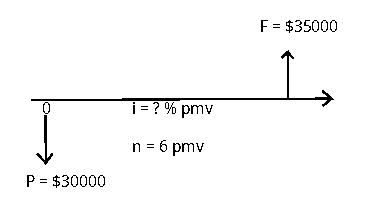
\includegraphics[scale=1.2]{1/capitulo1ejemplo1.pdf} }                                                                                         \\ \hline
%			%%%%%%%%%%%%% FIN INSERCIÓN DE IMAGEN
%			%%%%%FIN FLUJO DE CAJA
%			
%			
%			
%			%%%%% INICIO DECLARACIÓN FORMULAS
%			%%%%%%%%%%% INICIO TITULO
%			\rowcolor[HTML]{FFB183}
%			\multicolumn{3}{|c|}{\cellcolor[HTML]{FFB183}\textbf{4. Declaración de fórmulas}}                                                                                    \\ \hline
%			%%%%%%%%%%% FIN TITULO
%			%%%%%%%%%%% INICIO MATEMÁTICAS
%			
%			$F = P(1+in) \hspace{0.3cm} \textit{Valor futuro}$                   & \multicolumn{2}{c|}{$i = \frac{F}{nP}-\frac{1}{n} \hspace{0.3cm}\textit{Tasa de interés periódica}$}                      \\ \hline
%			%%%%%%%%%% FIN MATEMÁTICAS
%			%%%%%% INICIO DESARROLLO MATEMÁTICO
%			\rowcolor[HTML]{FFB183}
%			%%%%%%%%%%INICIO TITULO
%			\multicolumn{3}{|c|}{\cellcolor[HTML]{FFB183}\textbf{5. Desarrollo matemático}}                                                                                      \\ \hline
%			%%%%%%%%%% FIN TITULO
%			%%%%%%%%%% INICIO MATEMÁTICAS
%			 \multicolumn{3}{|c|}{$i =\frac{ COP 35{.}000}{6\cdot  COP 30{.}000}-\frac{1}{6}=0.2778$}                 \\ \hline
%			%%%%%%%%%% FIN MATEMÁTICAS
%			%%%%%% FIN DESARROLLO MATEMÁTICO
%			
%			\rowcolor[HTML]{FFB183}
%			\multicolumn{3}{|c|}{\cellcolor[HTML]{FFB183}\textbf{6. Respuesta}}    \\ \hline    
%			
%			\multicolumn{3}{|c|}{$i = 2.778\%pmv$} \\ \hline
%		\end{tabular}
%		%Se crean dos lineas en blanco para que no quede el siguiente texto tan pegado
%		\newline \newline
%	\end{center}
%\end{minipage}
%%%%%%%%%%%%%%%%%%%%%%%%%%%FIN EJERCICIO X %%%%%%%%%%%%%%%%%%%%%%%%%%%




\section{Interés anticipado (I$_{a}$)}
El Interés anticipado consiste en cobrar los intereses al principio del período.

\section{Tasa anticipada (d)}
La tasa anticipada es la que genera el interés anticipado y la representaremos por $"d"$, como veremos más adelante también se le denomina tasa de descuento.




%----------------------------------------------------------------------------------------
%	INDEX
%----------------------------------------------------------------------------------------
